\documentclass[a4paper,11pt]{article}

\usepackage[utf8]{inputenc} % Unicode support (Umlauts etc.)
\usepackage[ngerman]{babel} % Change hyphenation rules
\usepackage{ziffer} % , können in Zahlen verwendet werden ohne Formatierung kaputt zu machen
\usepackage[top=25mm,right=25mm,bottom=20mm,left=25mm,includefoot]{geometry} % Seitenränder

\usepackage[fleqn]{amsmath} % Formatierte Gleichungen
\usepackage{graphicx} % Grafiken
\usepackage{xcolor} % Farbe in Text
\usepackage{fancyhdr} % Seitenstil mit Kopfzeile etc.

\pagestyle{fancy}
\fancyhf{}
\lhead{Lösung Übungsblatt 2}
\rhead{Sascha Majewsky / Nils Hodys}
\rfoot{Seite \thepage}

\setlength{\parindent}{0cm} % Keine Einrückung der 1. Zeile eines Absatzes

\begin{document}
\section*{Aufgabe 1}

\subsection*{Entscheidungsvariablen}
\begin{flushleft}
$x_{B}$: Produktionsmenge Bananeneis in g pro Tag \\
$x_{H}$: Produktionsmenge Himbeereis in g pro Tag \\
$x_{E}$: Produktionsmenge Erdbeereis in g pro Tag \\
\end{flushleft}

\subsection*{Zielfunktion}
Die Zielfunktion ist in Euro je Gramm Eis angegeben und soll den Umsatz pro Tag maximieren.

\subsection*{LP}
\begin{align*}
    \text{max. } & z = 0,009x_{B} + 0,008x_{H} + 0,007x_{E} \\
    \\
    \text{s.t. } & x_{B} \le 3750 && \text{1500g Bananen ergeben 3750g Eis} \\
    & x_{B} + x_{H} \le 4000 && \text{400g Streusel ergeben 4000g Eis} \\
    & x_{H} \ge 1000 && \text{Spezialbestellung 1000g Eis} \\
    & x_{H} \le 5000 && \text{2000g Himbeeren ergeben 5000g Eis} \\
    & x_{E} \le 2000 && \text{Es stehen Erdbeeren für 2000g Eis zur verfügung} \\
    & x_{B} + x_{H} + x_{E} \le 6000 && \text{Es können max. 6000g produziert werden} \\
    & x_{B}, x_{H}, x_{E} \ge 0 && \text{Es kann keine negative Menge produziert werden} \\
\end{align*}

\subsection*{Lösung laut Solver}
\begin{flushleft}
$x_{B} = 3000$\\
$x_{H} = 1000$\\
$x_{E} = 2000$\\
\end{flushleft}

Umsatz bei optimaler Lösung (Euro pro Tag): $z = 49,00$ \\

\begin{centering}
	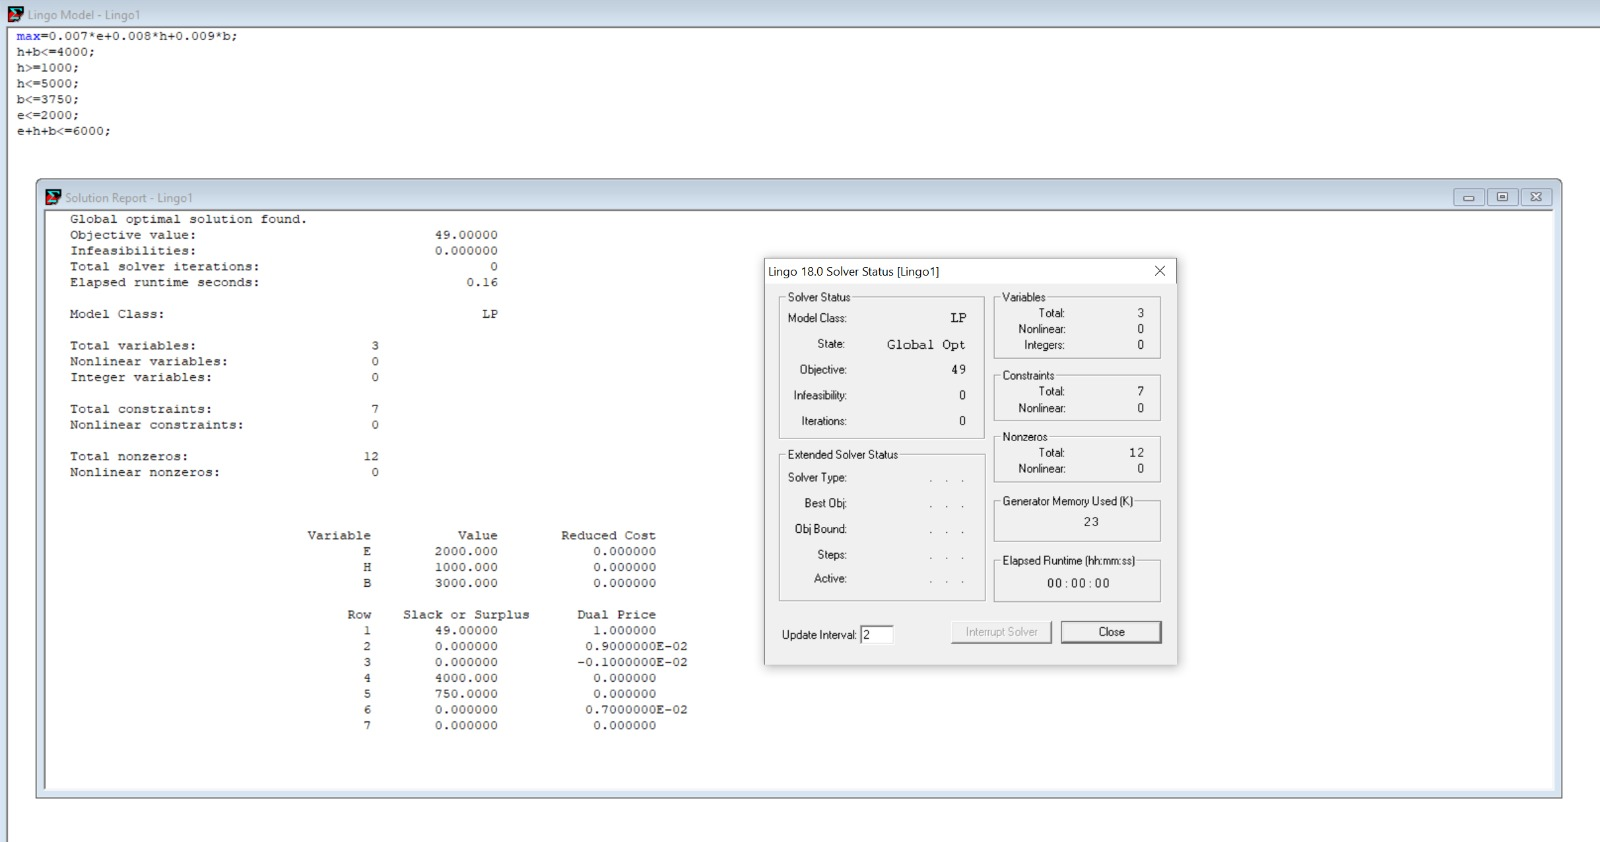
\includegraphics[width=1\linewidth]{src/solver_aufg_1.jpeg}
\end{centering}

\section*{Aufgabe 2}
Ausgangsmodell:
\begin{align*}
    \text{min. } & z = 6x_{1} + 3x_{2} - 2x_{3} \\
    \text{s.t. } & x_{3} + 2x_{1} \ge 6 \\
    & x_{1} + 6x_{2} = 2 \\
    & 5x_{3} + 2x_{2} \le -15 \\
    & x_{1}, x_{2} \ge 0 \\
\end{align*}

Freie Variable $x_{3}$ ersetzen:
\begin{align*}
    \text{min. } & z = 6x_{1} + 3x_{2} - 2x_{3}^{+} + 2x_{3}^{-}\\
    \text{s.t. } & x_{3}^{+} - x_{3}^{-} + 2x_{1} \ge 6 \\
    & x_{1} + 6x_{2} = 2 \\
    & 5x_{3}^{+} - 5x_{3}^{-} + 2x_{2} \le -15 \\
    & x_{1}, x_{2}, x_{3}^{+}, x_{3}^{-} \ge 0 \\
\end{align*}

Gleichung zu zwei Ungleichungen:
\begin{align*}
    \text{min. } & z = 6x_{1} + 3x_{2} - 2x_{3}^{+} + 2x_{3}^{-}\\
    \text{s.t. } & x_{3}^{+} - x_{3}^{-} + 2x_{1} \ge 6 \\
    & x_{1} + 6x_{2} \le 2 \\
    & x_{1} + 6x_{2} \ge 2 \\
    & 5x_{3}^{+} - 5x_{3}^{-} + 2x_{2} \le -15 \\
    & x_{1}, x_{2}, x_{3}^{+}, x_{3}^{-} \ge 0 \\
\end{align*}

Min-Zielfunktion zu Max-Zielfunktion:
\begin{align*}
    \text{max. } & z = -6x_{1} - 3x_{2} + 2x_{3}^{+} - 2x_{3}^{-}\\
    \text{s.t. } & x_{3}^{+} - x_{3}^{-} + 2x_{1} \ge 6 \\
    & x_{1} + 6x_{2} \le 2 \\
    & x_{1} + 6x_{2} \ge 2 \\
    & 5x_{3}^{+} - 5x_{3}^{-} + 2x_{2} \le -15 \\
    & x_{1}, x_{2}, x_{3}^{+}, x_{3}^{-} \ge 0 \\
\end{align*}

Ungleichungen zu Gleichungen mit Schlupfvariablen:
\begin{align*}
    \text{max. } & z = -6x_{1} - 3x_{2} + 2x_{3}^{+} - 2x_{3}^{-}\\
    \text{s.t. } & x_{3}^{+} - x_{3}^{-} + 2x_{1} - x_{4} = 6 \\
    & x_{1} + 6x_{2} + x_{5} = 2 \\
    & x_{1} + 6x_{2} - x_{6} = 2 \\
    & 5x_{3}^{+} - 5x_{3}^{-} + 2x_{2} + x_{7} = -15 \\
    & x_{1}, x_{2}, x_{3}^{+}, x_{3}^{-}, x_{4}, x_{5}, x_{6}, x_{7} \ge 0 \\
\end{align*}

\section*{Aufgabe 3}
Ausgangsmodell:
\begin{align*}
    \text{max. } & z = 5x_{1} + 15x_{2} + 10x_{3} \\
    \text{s.t. } & x_{3} \le 10 \\
    & x_{3} + x_{2} \le 20 \\
    & 2x_{3} + 5x_{1} \le 50 \\
    & 4x_{1} + 2x_{2} \le 70 \\
    & x_{1}, x_{2}, x_{3} \ge 0 \\
\end{align*}

\begin{itemize}
    \item Keine freien Variablen
    \item Nur Ungleichungen
    \item Bereits eine Max-Zielfunktion
\end{itemize}

\vspace{4mm}
    
Ungleichungen zu Gleichungen mit Schlupfvariablen:
\begin{align*}
    \text{max. } & z = 5x_{1} + 15x_{2} + 10x_{3} \\
    \text{s.t. } & x_{3} + x_{4} = 10 \\
    & x_{3} + x_{2} + x_{5} = 20 \\
    & 2x_{3} + 5x_{1} + x_{6} = 50 \\
    & 4x_{1} + 2x_{2} + x_{7} = 70 \\
    & x_{1}, x_{2}, x_{3}, x_{4}, x_{5}, x_{6}, x_{7} \ge 0 \\
\end{align*}

$\to$ Modell liegt jetzt in Standardform vor.

\subsection*{Simplex II}
\begin{align*}
    \text{max. } z &= 5x_{1} + 15x_{2} + 10x_{3} \\
    x_{4} &= 10 - x_{3} \\
    x_{5} &= 20 - x_{2} - x_{3} \\
    x_{6} &= 50 - 5x_{1} - 2x_{3} \\
    x_{7} &= 70 - 4x_{1} - 2x_{2} \\
    & x_{1}, x_{2}, x_{3}, x_{4}, x_{5}, x_{6}, x_{7} \ge 0 \\
\end{align*}

Basislösung: $x_{4}=10; x_{5}=20; x_{6}=50; x_{7}=70;$ \\
$\to$ Zulässig, weil keine NBV mit negativem Wert \\
$\to$ Nicht degeneriert, weil keine NBV gleich 0 \\

Iteration 1: \\
{\color{red} Selektiere größten positiven NBV Koeffizient (15)}
\begin{align*}
    \text{max. } z &= 5x_{1} + {\color{red}15x_{2}} + 10x_{3} && \text{Quotiententest} \\
    x_{4} &= 10 - x_{3} && \big| x_{2} \le \infty \\
    x_{5} &= 20 - {\color{red}x_{2}} - x_{3} && \big| x_{2} \color{red} \le 20  \text{ (Minimale Beschränkung)} \\
    x_{6} &= 50 - 5x_{1} - 2x_{3} && \big| x_{2} \le \infty \\
    x_{7} &= 70 - 4x_{1} - {\color{red}2x_{2}} && \big| x_{2} \le 70:2=35 \\
    & x_{1}, x_{2}, x_{3}, x_{4}, x_{5}, x_{6}, x_{7} \ge 0 \\
    \\
    &&& \text{Termumformung:} \\
    &&& x_{5}= 20 -x_{2} -x_{3} &&\big| + x_{2} \\
    &&& x_{2} + x_{5}= 20 -x_{3} &&\big| - x_{5} \\
    &&& x_{2} = 20 -x_{3} - x_{5}
\end{align*}

Iteration 2: \\
{\color{red} Selektiere größten positiven NBV Koeffizient (5)}
\begin{align*}
    \text{max. } z &= 300 + {\color{red}5x_{1}} - 5x_{3} - 15x_{5} && \text{Quotiententest} \\
    x_{4} &= 10 - x_{3} && \big| x_{1} \le \infty \\
    x_{2} &= 20 - x_{3} - x_{5} && \big| x_{1} \le \infty \\
    x_{6} &= 50 - {\color{red}5x_{1}} - 2x_{3} && \big| x_{1} \le 10 \\
    x_{7} &= 30 - {\color{red}4x_{1}} + 2x_{3} + 2x_{5} && \big| \color{red} x_{1} \le 30:4=7,5 \text{ (Minimale Beschränkung)} \\
    & x_{1}, x_{2}, x_{3}, x_{4}, x_{5}, x_{6}, x_{7} \ge 0 \\
    \\
    &&& \text{Termumformung:} \\
    &&& x_{7}= 30 -x_{4} +2x_{3} +2x_{5} &&\big| + 4x_{1} \\
    &&& 4x_{1} + x_{7} = 30 +2x_{3} +2x_{5} &&\big| - x_{7} \\
    &&& 4x_{1} = 30 +2x_{3} +2x_{5} - x_{7} &&\big| :4 \\
    &&& x_{1} = 7,5 +0,5x_{3} +0,5x_{5} - 0,25x_{7} \\
\end{align*}

Iteration 3:
\begin{align*}
    \text{max. } z &= {\color{teal}337,5} - 2,5x_{3} - 12,5x_{5} - 1,25x_{7} \\
    x_{4} &= 10 - x_{3} \\
    x_{2} &= {\color{teal}20} - x_{3} - x_{5} \\
    x_{6} &= 12,5 - 4,5x_{3} - 2,5x_{5} + 1,25x_{7} \\
    x_{1} &= {\color{teal}7,5} + 0,5x_{3} + 0,5x_{5} - 0,25x_{7} \\
    & x_{1}, x_{2}, x_{3}, x_{4}, x_{5}, x_{6}, x_{7} \ge 0 \\
\end{align*}

$\to$ \textbf{Optimale Lösung bei:}
\begin{align*}
    x_{1} &= 7,5 \\
    x_{2} &= 20 \\
    x_{3} &= 0 \\
    z &= 337,5 \\
\end{align*}

\end{document}